\usepackage[authoryear,round]{natbib}
\usepackage{multirow}

\newcommand{\sheetnum}{%
	02
}
%\setcounter{section}{\sheetnum-3}
\newcommand{\tutorialtitle}{%
    Hebbian Learning - Online Principal Component Analysis
}
\newcommand{\tutorialtitleshort}{%
	Online PCA
}
% for slides
\subtitle{\sheetnum \tutorialtitle}

\maxdeadcycles=1000 % Workaround for ! Output loop---100 consecutive dead cycles because of too many figures

% The following use of algroithms does not work well with the notes:
%
%
%
%
% instead use the following for your algorithms:
%
%\begin{figure}[!t]
%\removelatexerror
%\begin{algorithm}[H]
    % your algo here
    %\label{alg:algolabel}
    %\caption{algocaption}
%\end{algorithm}
%\end{figure}
%\begin{algorithm}
% Below is the definition for the command \removelatexerror:
\makeatletter
\newcommand{\removelatexerror}{\let\@latex@error\@gobble}
\makeatother

\begin{document} %%%%%%%%%%%%%%%%%%%%%%%%%%%%%%%%%%%%%%%%%%%%%%%%%%%%%%%

%\chapter{T\sheetnum} % doesn't work with scrartcl

\sheet{\sheetnum}{\tutorialtitleshort}

\ttopic{\tutorialtitle}

\columnratio{0.2,0.8}\textbf{}
\begin{paracol}{2}
%\setlength{\columnseprule}{0.1pt}
%\setlength{\columnsep}{5em}

\begin{rightcolumn}

% notes version will ignore it
\begin{frame}
\titlepage
\end{frame}

\begin{frame}
\tableofcontents[hideallsubsections]
\end{frame}

\newpage

\mode<all>

\section{PCA: Recap}

\begin{frame}{\secname}

\begin{itemize}
\item requires centering the data
\item \notesonly{eigendecomposition of $\text{Cov}(\vec X)$}\slidesonly{$\text{eig(}\text{Cov}(\vec X))$}, alternatively: SVD($\vec X$)
\item sensitive to the scales of the individual variables
\item deterministic, insensitive to the order of the observations
\item Applications: dimensionality reduction, outlier detection, whitening
\item limited to linear correlations
\item will be referred to as ``standard'' or ``batch'' PCA.
\end{itemize}

\end{frame}

\begin{frame}{Non-stationary data}

\pause

\svspace{35mm}

\question{What are the implications of computing PCA on \emph{non-stationary} data?}

\pause

- We need an online method for computing the directions of highest variance that adapts to possible changes in this direction over time.

\end{frame}

\section{Hebbian Learning}

\mode<presentation>{
\begin{frame} 
    \begin{center} \huge
        \secname
    \end{center}
	\begin{center}
	\textit{``Neurons that fire together wire together.''} - Donald Hebb
	\end{center}
	\svspace{10mm}
\end{frame}
}

\mode<article>{
\begin{center}
\textit{``Neurons that fire together wire together.''} - Donald Hebb
\end{center}
}

\begin{frame}
\frametitle{\secname\only<4->{: What is the neuron learning?}}

\svspace{-3mm}

\only<1-3>{
\begin{center}
\includegraphics[width=4cm]{img/section2_fig5_a}
\captionof{figure}{A linear neuron}
\end{center}
}

\begin{itemize}
\item[] 
\only<1-3>{
Observations:\notesonly{\\}
\begin{equation}
\big\{ \vec{x}^{(\alpha)} \in \R^N \big\},\; \alpha = 1, \ldots, p,
\end{equation}
\notesonly{
\begin{equation}
\big(x_1, x_2,\ldots,x_j,\ldots,x_N\big)^\top = \vec{x} \in \R^N
\end{equation}
}

\item[] Assumption: centered data\notesonly{,
\begin{equation}\E\lbrack \vec x \rbrack = \vec 0
\end{equation}}

}

\mode<presentation>{
\only<2>{
\begin{center}
\includegraphics[width=2.5cm]{img/meme_centeronemoretime}
\end{center}
}
}
\only<3->{
\item[] Response: 
\begin{equation}
y = \sum_{j=1}^{N} w_j x_j = \vec w^{\top} \vec x \only<4>{= \lVert \vec w \rVert \, \lVert \vec x \rVert \cos \theta}
\end{equation}

\item[] We don't really have a desired output for the network.\\
\item[] However, we can interpret its response $y$.\\
}
\only<4>{

\begin{center}
\includegraphics[width=4.5cm]{img/wxangle}
\end{center}

The inner product yields a higher value whenever $\vec x$ is ``close'' to $\vec w$.
Therefore, $y$ measures similarity between $\vec x$ and $\vec w$.
A large value of $y$ means that the network ``recognizes'' the stimulus $\vec x$.
}
\end{itemize}

\end{frame}

\newpage

\subsection{Motivation for Hebbian learnig}

\begin{frame}{\subsecname}

\begin{itemize}
\item We can use this to build associative memory (i.e. correlation learning).
\item Applicable to non-stationary data.
\item More importantly, a single linear neuron 
can organize itself such that its synaptic weights converge to a filter 
for the \slidesonly{first PC}\notesonly{\emph{first principle component}} \citep{oja1982simplified}.

\pause

\mode<presentation>{
\svspace{5mm}
    \begin{center}
		\includegraphics[width=3cm]{img/meme_hebbian}
    \end{center}
}

\end{itemize}

\end{frame}

\subsection{The Hebbian learning rule}

\begin{frame}{\subsecname}
\begin{equation}
\vec w(t+1) = \vec w(t) + \underbrace{\varepsilon~y(\vec x^ {(\alpha)}; \vec w(t)) \vec x^{(\alpha)}}_{= \Delta \vec w}
\end{equation}
where $\varepsilon$ is the \emph{learning rate}.\\

\underline{The consequences of using this update rule in simulation:}\\

\begin{enumerate}
\item Divergence.\\
As $t \rightarrow \infty$ \qquad $\leadsto |\vec{w}| \rightarrow \infty$\\

\pause 

\notesonly{
\question{How does nature deal with the divergence problem?}
}

\mode<presentation>{
\only<2>{
\svspace{5mm}
    \begin{center}
		\includegraphics[width=3.5cm]{img/meme_diverges}
    \end{center}
}
}

\pause

\item $\vec{e}_{\mathrm{w}} = \frac{\vec{w}}{|\vec{w}|}$ 
\end{enumerate}

\end{frame}


\mode*

\clearpage

\mode<all>
\section{Oja's rule}

\mode<presentation>{
\begin{frame} 
    \begin{center} \huge
        \secname
    \end{center}
	%\begin{center}
	%Dealing with the diverging hebbian rule\\
	%through implicit normalization
	
	%\end{center}
	\svspace{5mm}
    \begin{center}
		\includegraphics[width=4cm]{img/meme_oja}
    \end{center}
\end{frame}
}

\begin{frame}{\secname}

Modify the update rule such that 
\begin{itemize}
\item it contains an 
\emph{implicit normalization} to prevent divergence and 
\item $\vec w$ still converges to the direction of the first PC.
\end{itemize}

\question{How?}

-By adding a \emph{decay term} to the update rule.

\begin{block}{Oja's rule:}
\begin{equation}
	\Delta {w}_j = \varepsilon~y_{ \big( \vec{x}^{(\alpha)}; \vec{w}
		\big) } \bigg\{ 
			\underbrace{ x_j^{(\alpha)} }_{
				\substack{	\text{Hebbian} \\
						\text{learning} }}
			- 
					\underbrace{
	y_{ \big( \vec{x}^{(\alpha)}; \vec{w} \big) } {w}_j
	}_{\text{decay term}}
			\bigg\}
\end{equation}
\end{block}

\end{frame}

\subsection{Alternative: Explicit normalization}

\mode<presentation>{   
\begin{frame}{Alternative to Oja's rule}

All Oja's rule does is:

\begin{itemize}
\item provide an
\emph{implicit normalization} to prevent divergence and 
still 
\item have $\vec w$ converge to the direction of the first PC.
\end{itemize}
	%\begin{center}
	%Dealing with the diverging hebbian rule\\
	%through implicit normalization
	%\pause
	%\end{center}
	\svspace{5mm}
    \begin{center}
		\includegraphics<2>[width=2cm]{img/smart_cookie}
		\includegraphics<3>[width=4cm]{img/meme_normalization}
    \end{center}
\end{frame}
}


\begin{frame}{\subsecname}

\begin{block}{Explicit normalization} 
i.e. keep $|\vec w| = 1$ after each step by normalizing it.

\begin{equation}
	\vec{w}(t+1) = 
    \frac{\vec w(t) + \Delta \vec w}{|\vec w(t) + \Delta \vec w|} 
    = \frac
    {\overbrace{\vec{w}(t) + {\only<3->{\color{blue}}\varepsilon y(\vec{x}^{(\alpha)}; \vec{w}(t))~\vec{x}^{(\alpha)}}}^{\text{Hebbian learning}}}
    {\underbrace{\left| \vec{w}(t) + \varepsilon y(\vec{x}^{(\alpha)}; \vec{w}(t))~\vec{x}^{(\alpha)} \right|}_{\text{Euclidean weights normalization}}}
    \label{eq:explicitnorm}
\end{equation}

\only<2>{
For the $j$-th component:\\
\begin{equation}
    w_j(t+1) = \frac
    {w_j(t) + \varepsilon y(\vec{x}^{(\alpha)}; \vec{w}(t))~x_j^{(\alpha)}}
    {\sqrt{ \sum_{k=1}^{N} \left( w_k(t) + \varepsilon y(\vec{x}^{(\alpha)}; \vec{w}(t))~{x_k}^{(\alpha)} \right)^2}}
\end{equation}

}



\end{block}

\notesonly{ 
Keep in mind that the above explicit normalization in \eqref{eq:explicitnorm}}
\only<3>{
uses the \textcolor{blue}{original hebbian update rule}
\notesonly{
$\color{blue}\Delta \vec w = \varepsilon y(\vec x^ {(\alpha)}; \vec w(t)) 
~\vec x^{(\alpha)}$} \underline{without} the decay term.}\notesonly{\\
If we were using the decay term, we wouldn't need an explicit normalization.
}

\only<4>{
\slidesonly{

    \begin{center}
		\includegraphics[width=3.5cm]{img/meme_decay}
    \end{center}
}
}
\end{frame}

\begin{frame}

\question{Does Oja's rule give different results than the explicit normalization?}\\

\notesonly{- No.\\}

\mode<presentation>{
\svspace{5mm}
\begin{center}
	
\includegraphics[width=3.5cm]{img/meme_ojaexplicit-same}
\end{center}
}

\pause

In the excercise sheet you will demonstrate that for small $\varepsilon$ the explicit normalization can be reduced to Oja's rule using a Taylor expansion around $\varepsilon = 0$ and neglecting terms of second or higher order in $\varepsilon$. 

\end{frame}

\mode*

\clearpage

\mode<all>

\section{Online-PCA}

\mode<presentation>{
\begin{frame} 
    \begin{center} \huge
        \secname
    \end{center}
\end{frame}
}

\begin{frame}
W\notesonly{e have established that w}e can use Hebbian learning (Oja's rule to prevent divergence) 
to find the direction of the first \notesonly{principle component $\vec e_1$}\slidesonly{PC} in the data. \\

\pause

Note that
\begin{align}\text{with} \quad \vec w &= \vec e_1\\
\text{follows} \quad y &= \vec e_1^\top \vec x =: a_1
\end{align}

\question{What else is there to do?}

\pause

- Find all other PCs

\end{frame}

\begin{frame}{Only}\frametitle{\secname}
%\only<1>{
\svspace{-5mm}
\begin{center}
%\includegraphics<1>[width=4cm]{img/section2_fig5_b_2}
%\slidesonly{
%\includegraphics<2>[width=4cm]{img/section2_fig5_b_2_blue}
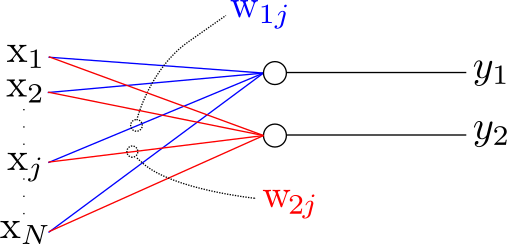
\includegraphics[width=4cm]{img/section2_fig5_b_2_blue-red}
%}
\only<1>{
\captionof{figure}{A neural network}
}
\end{center}
\svspace{-3mm}

\only<1>{
We proceed to learning the next PC by doing the following:
}
\begin{enumerate}
\item<only@1> Denote the network's response with $y_1$ and its weight vector as $\color{blue}\vec w_1$, knowing that ${\color{blue}\vec w_1} = \vec e_1$.
\item<only@1> Add a second neuron $y_2$ to our network. This neuron will come with its own randomly initialized weight vector $\color{red}\vec w_2$.
\item<only@1,2> Resume feeding new data points into the network computing its response $y_1$ and $y_2$.
\item<only@2,3> We exploit that the PCs form an \emph{orthonormal basis}, specifically, we obtain a projection of $\vec x$ 
into the subspace orthogonal to $\vec e_1$\notesonly{ that is the first PC}:
\begin{align}
\hat x_j &= x_j - {\color{blue} w_{1j}} \, y_1 \only<2>{
\intertext{Recall: ${\color{blue}\vec w_1} = \vec e_1 \rightarrow \; y = \vec e_1^\top \vec x =: a_1$}}
         \only<2>{&}= x_j - a_1 (\vec e_1)_j
         \label{eq:projorth}
\end{align}

%\slidesonly{
%\only<2>{
%\placeimage{11}{7}{img/section2_fig5_b_2_blue}{width=4cm}
%}
%\only<3>{
%\placeimage{11}{7}{img/section2_fig5_b_2_blue-red}{width=4cm}
%}
%}
\notesonly{where $\color{blue}w_{1j}$ is the weight of the connection between $\hat x_j$ and the neuron $y_1$,}
\item<only@3-> Apply Oja's rule on $\color{red}\vec w_2$.

For \underline{stationary} data: No need to apply updates to $\color{blue}\vec w_1$ anymore, since it has already converged to $\vec e_1$.\notesonly{ Applying the update to $\color{blue}\vec w_1$ would only yield negligible change in the case of stationary data.}
\slidesonly{Further updates would lead to negligible change.}
 
\item<only@3-> Continue feeding observations until $\color{red}\vec w_2$ has converged.
\item<only@3-> On convergence, ${\color{red}\vec w_2} = \vec e_2$.
\end{enumerate}

\end{frame}

\begin{frame}


\begin{center}
\includegraphics[width=4cm]{img/othogonality_novelty_less}
\captionof{figure}{A graphical interpretation}
\end{center}

\notesonly{\label{eq:projorth} }using vector notation:
\begin{align}
\hat {\vec x} &= \vec x - \vec w_1 \, y_1\\
			&= \vec x - a_1 \vec e_1
\end{align}

\pause

We get the remaining PCs by repeating the above except, that we project 
the data onto the subspace orthogonal to \textbf{all previous} PCs.\\
(cf. lecture slides 1.2 ``Learning: Oja's rule \& Gram-Schmidt orthonormalization'')

\end{frame}


\mode*

\clearpage

\mode<all>
\section{Applying Online-PCA}

\subsection{Novelty filter}

\mode<presentation>{
\begin{frame} 
    \begin{center} \huge
        \secname
    \end{center}
    Same as PCA
    Example Application: Novelty filter
\end{frame}
}

\begin{frame}

Applying online PCA for detecting outliers - identifying observations with unusual features. 

\slidesonly{
\begin{center}
	\includegraphics[width=0.3\textwidth]{img/meme_outlier_novelty}%
\end{center}
}
Calling it an ``outlier'' or a point with `novel'' features depends on the context. But they are essentially the same.

Can also be done using ``standard'' or ``batch'' PCA.

\end{frame}

\begin{frame}\frametitle{\subsecname}

\only<1>{
\question{What are the PCs with smallest eigenvalues useful for?}\\
}

\pause 
\question{Can we modify online PCA by learning the PCs in reverse order (i.e. PCs with smallest eigenvalues first?}\\

\only<3>{
\slidesonly{
\begin{center}
	\includegraphics[width=0.3\textwidth]{img/meme_yesyoucan}%
\end{center}
}
}

\notesonly{- Yes by using the \emph{Anti-Hebbian rule}}

\end{frame}

\subsubsection{Novelty Filter with normalization}

\begin{frame}\frametitle{\subsubsecname}

	\begin{block}{Anti-Hebbian rule:}
				\begin{equation}
				\Delta w_j = \overbrace{-}^{\substack{	\text{``Anti''-} \\ \text{Hebbian} }} \varepsilon y^{(\alpha)} x_j^{(\alpha)}
				\end{equation}
	\end{block}
	
	Not prone to diveregence but $\vec w$ will become smaller and smaller.
	\pause
	
	Normalization needed:
	
	\begin{equation}
		\Delta \vec{w} = - \varepsilon  \frac{y^{(\alpha)} \left\{ \vec{x}^{(\alpha)} - y^{(\alpha)} \vec{w} \right\}}{|{\vec{w} - \varepsilon y^{(\alpha)} \left\{ \vec{x}^{(\alpha)} - y^{(\alpha)} \vec{w} \right\}}|}
	\end{equation}
	
	Anti-Hebbian version of Oja's rule also (cf. lecture slides)

\end{frame}


\begin{frame}

\question{Are the other ways to learn a novelty filter without PCA?}

\pause

- Yes, through linear regression:

\end{frame}

\newpage

\subsubsection{Novelty Filter and linear regression}

\begin{frame}\frametitle{\subsubsecname}
	\svspace{-3mm}

\begin{center}
\notesonly{
\hspace{-10mm}
}
\begin{minipage}{0.45\textwidth}
	\begin{center}
		\includegraphics[width=0.6\textwidth]{img/linear_regression}%
		%\captionof{figure}{Ordinary least squares}
	\end{center}
	\svspace{-5mm}
	
	\begin{block}{ordinary least squares:}
	\svspace{-2mm}
		\begin{equation}
		\frac{1}{p} \sum_{\alpha = 1}^{p} \left( {\color{blue}e^{(\alpha)}} \right)^2 \eqexcl \min_{\vec w}
		\end{equation}
	\end{block}
\end{minipage}
\slidesonly{
\hspace{5mm}
}
\notesonly{
\hspace{2mm}
}
\visible<2>{
\begin{minipage}{0.45\textwidth}
	\begin{center}
		\includegraphics[width=0.6\textwidth]{img/linear_regression_a}%
		%\captionof{figure}{Total least squares}
	\end{center}
	\svspace{-5mm}
	
	\begin{block}{total least squares:}
	\svspace{-2mm}
			\begin{equation}
				\frac{1}{p} \sum_{\alpha =1}^{p} \left( {\color{magenta}d^{(\alpha)}} \right)^2 \eqexcl \min_{\vec w}
			\end{equation}
		\end{block}
\end{minipage}
}
\end{center}

\svspace{-1mm}

\underline{Assumptions}:\\




\svspace{-1mm}

\notesonly{
	\resizebox{0.8\textwidth}{!}{%
	\begin{tabular}{|l|l|}
	\hline 
	ordinary least squares		  &  total least squares
	\\ \hline
	$\leadsto$ noise along $x_2$ only		  &  $\leadsto$ same variance noise\\ \hline
	$\leadsto$wrong if data points are also noisy along $x_1$ & $\leadsto$ centered data $\rightarrow \vec{w}^\top\vec{x} = 0$ 
	\\ \hline
	\end{tabular}%
	}
}

\slidesonly{	
\begin{center}
\begin{minipage}{\slidesonly{0.45}\notesonly{0.3}\textwidth}
		\begin{itemize}
			\itl noise along $x_2$ only
			\itl wrong if data points are also noisy along $x_1$
		\end{itemize}
\end{minipage}
\hspace{5mm}
$\Bigg|$
\visible<2>{
\begin{minipage}{\slidesonly{0.45}\notesonly{0.3}\textwidth}
		\begin{itemize}
			\itl same variance noise
			\itl centered data $\rightarrow \vec{w}^\top\vec{x} = 0$ 
		\end{itemize}
\end{minipage}
}
\end{center}
}


%- (cf. slides 1.2 \#23-\#25.)


\end{frame}

\section{PCA vs. online PCA}

\begin{frame}\frametitle{\secname}

\underline{Common properties:}

\begin{itemize}
\item assume the data is centered
\item sensitive to the scales of the individual variables
\item for stationary data, both converge to the same solution
\item limited to linear correlations between the variables (cf. Kernel PCA to account for non-linear correlations)
\end{itemize}

\pause

\question{PCA vs. online PCA. How to choose?}\\

\only<2>{
\slidesonly{
\begin{center}
	\includegraphics[width=0.2\textwidth]{img/meme_pca_vs_online_pca}%
\end{center}
}
}

\pause

- staionarity of the data\\
- can I fit all the data into memory?


\end{frame}

\mode*

\section{References}
\begin{frame}[allowframebreaks] \frametitle{References}
	\scriptsize
	\bibliographystyle{plainnat}
	\bibliography{bibliography}
\end{frame}

\end{rightcolumn}
\end{paracol}

\end{document}
